\chapter{Addendum} % Main chapter title
%\addcontentsline{toc}{chapter}{Listings}
\label{chapter-addendum}

This chapter contains source code listings that are too long to be included in-line in the previous chapters.

\section{iDigBio presentation}

This section contains details of the webinar accompanying Chapter~\ref{chapter-case-study}.

A video recording of the presentation is available \href{http://idigbio.adobeconnect.com/p7sg0aym3e3/}{from iDigBio}. More information can be found in the \href{http://www.idigbio.org/content/online-direct-import-specimen-records-idigbio-infrastructure-taxonomic-manuscripts}{webinar information page over at iDigBio}. The slides of the presentation are attached as supplementary files and are deposited in \href{http://www.slideshare.net/ViktorSenderov/online-direct-import-of-specimen-records-from-idigbio-infrastructure-into-taxonomic-manuscripts}{Slideshare}\footnote{The electronic version of the PDF contains clickable links to the video, notes, and slides.}.

During the presentation we conducted a poll about the occupation of the attendees, the results of which are summarized in Fig.~\ref{fig:webinar-poll}. Of the participants who voted, about a half were scientists, mostly biologists, while the remainder were distributed across IT specialists and librarians, with 20\% ``Other.'' The other categories might have been administrators, decision-makers, non-biology scientists, collections personnel, educators, etc.

\begin{figure}
\centering
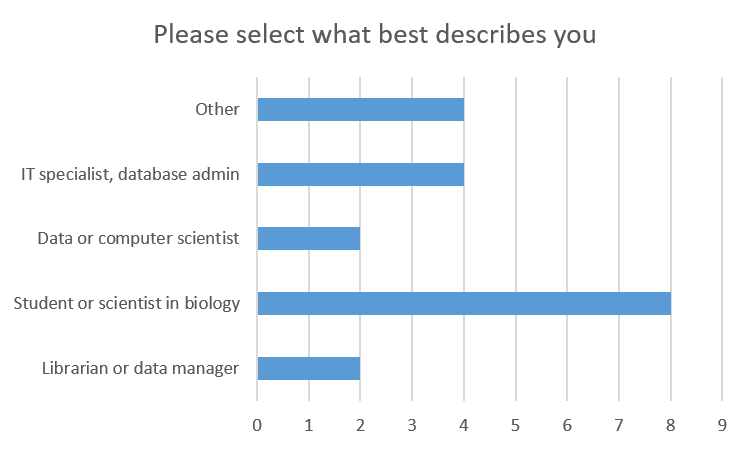
\includegraphics[width=\textwidth]{Figures/webinar-pool}
\decoRule
\caption{Poll results about composition of audience during live participation..}
\label{fig:webinar-poll}
\end{figure}

At the end of the presentation, very interesting questions were raised and discussed. For details, see the ``Results and discussion'' section of this paper.

Larry Page, Project Director at iDigBio, wrote: ``This workflow has the potential to be a huge step forward in documenting use of collections data and enabling iDigBio and other aggregators to report that information back to the institutions providing the data.''

Neil Cobb, a research professor at the Department of Biological Sciences at the Northern Arizona University, suggested that the methods, workflows and tools addressed during the presentation could provide a basis for a virtual student course in biodiversity informatics.